\documentclass[12pt]{article}
\usepackage[utf8]{inputenc}

%%% PAGE DIMENSIONS
\usepackage{geometry} % to change the page dimensions
\geometry{margin=0.5in}

\usepackage{graphicx} 

%%% PACKAGES
\usepackage{booktabs} 
\usepackage{array} 
\usepackage{paralist}
\usepackage{verbatim} 
\usepackage{subfig} 
\usepackage{longtable}
\usepackage{listings}
\usepackage{amsmath}
\usepackage{pdfpages}


%%% HEADERS & FOOTERS
\usepackage{fancyhdr}
\pagestyle{fancy} 
\renewcommand{\headrulewidth}{0pt} 
\lhead{ATSC 500}\chead{}\rhead{Eve Wicksteed}
\lfoot{}\cfoot{\thepage}\rfoot{}

%%% TABLE FONT
\usepackage{etoolbox}
\AtBeginEnvironment{longtable}{\sffamily}
\AtBeginEnvironment{table}{\sffamily}

%%% CODE FONT
\newcommand{\code}[1]{\texttt{#1}}

%%% SECTION TITLE APPEARANCE
\usepackage{sectsty}
\allsectionsfont{\sffamily\mdseries\upshape} 

%%%
\title{A COMPARISON OF MODEL DATA AND OBSERVATIONS IN THE ATMOSPHERIC BOUNDARY LAYER}
%\subtitle{ATSC 500 - Boundary Layer Final Project}
\author{Eve Wicksteed}
\date{January 2020}

\begin{document}

\maketitle

\section{Introduction}


It’s important for models to be able to simulate the atmosphere fairly accurately for them to 
be useful to us. The boundary layer (BL) is one of the many things a model should be able to 
simulate. In order to simulate the boundary layer, models are required to have planetary boundary 
layer (PBL) schemes in which they parameterize boundary layer processes.  These parameterizations 
need to be made because models are not able to resolve fluxes at the required spatial scales 
for the BL.  This is because the length-scales of eddies are smaller than the model grid spacing 
(which is normally somewhere between 1 and 4 km). Accuracy in PBL schemes is important because 
uncertainty and inaccuracies in these forecasts can have impacts on larger scale phenomena 
(Coniglio et al, 2013).

In order to determine the ability of a model to simulate the BL, I will compare the results of 
model simulations to observations taken in the boundary layer by atmospheric soundings (sondes). 
In particular I compare potential temperature predictions under different atmospheric stability 
conditions for different times of day. 


\section{Study Area}

My area of study is Cape Town, South Africa (33° 55’ 31’’ S, 18° 25’ 26’’ E). I have chosen 
this location because I am familiar with the area and the weather and thus I am able to have 
an intuition of the physical processes represented by the data. Cape Town’s time zone is GMT+2. 
This means that the data at 00z and 12z correspond to 02:00 and 14:00 local time, respectively, 
and provides examples of soundings both during the day and at night. Although I have specifically 
chose Cape Town for this project, the methodology could easily be applied to other locations 
given available data.

\graphicspath{ {/Users/catherinemathews/UBC/a500_notebooks/project/figures/new_to_use/} }

\begin{figure}[h]
    \centering
    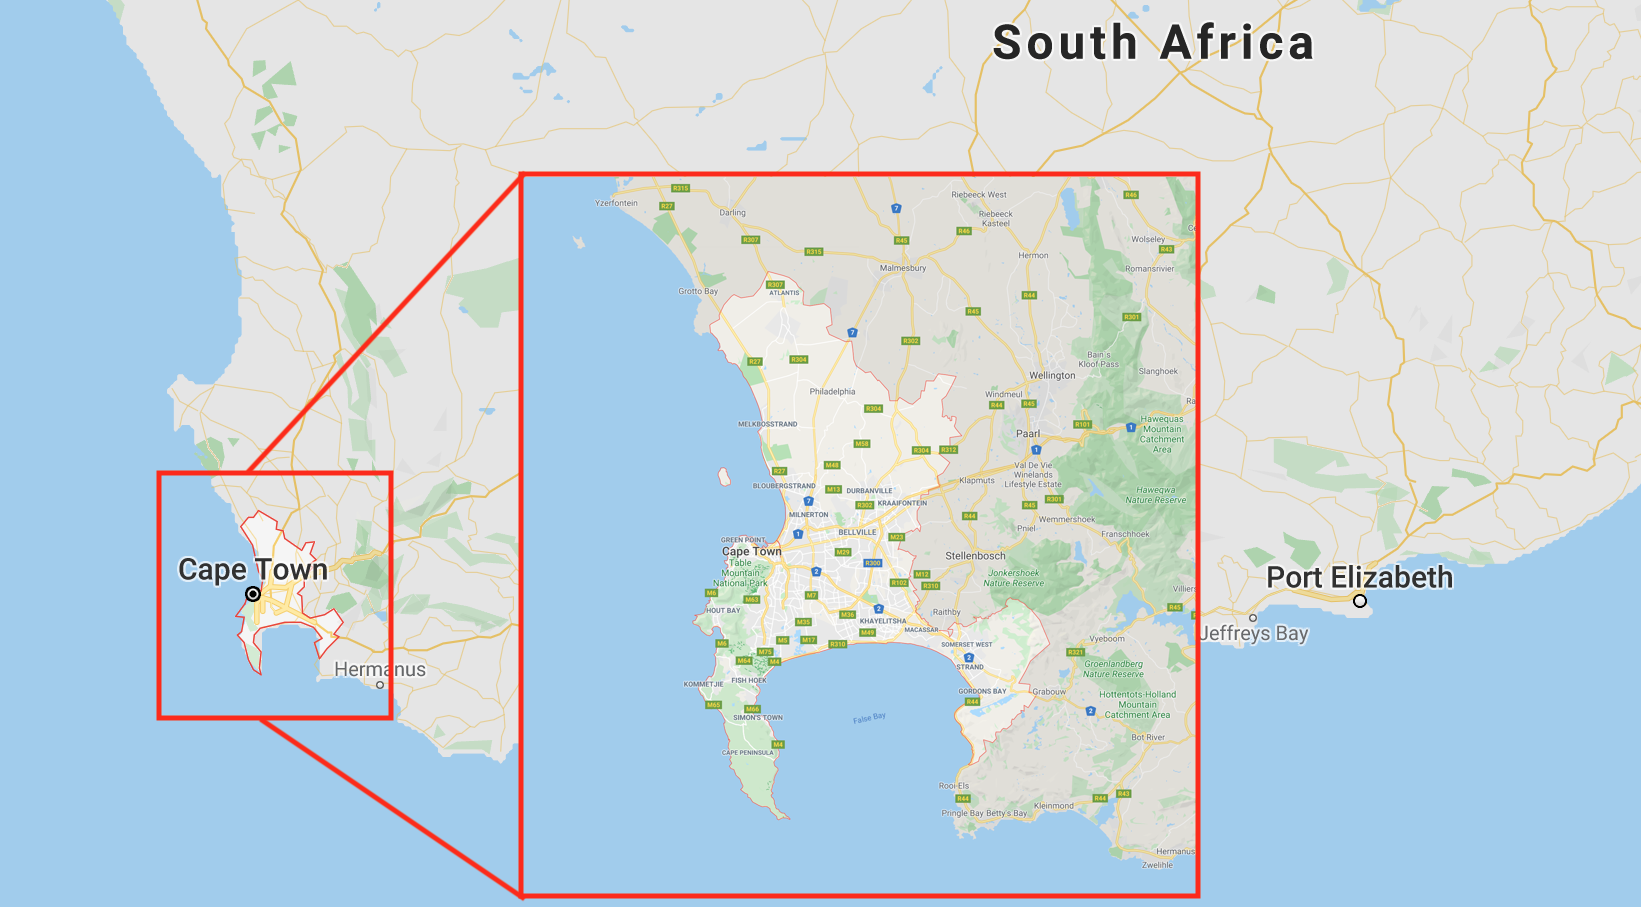
\includegraphics[width=\textwidth]{CT_map_crop.png}
    \caption{Map of Cape Town, South Africa (Google Maps, 2019)}
    \label{fig:map}
\end{figure}

\section{Data}

For this study I use the potential temperature variable to compare the 
results of model output to observations. 

\subsection{Model}

\begin{figure}[h]
    \centering
    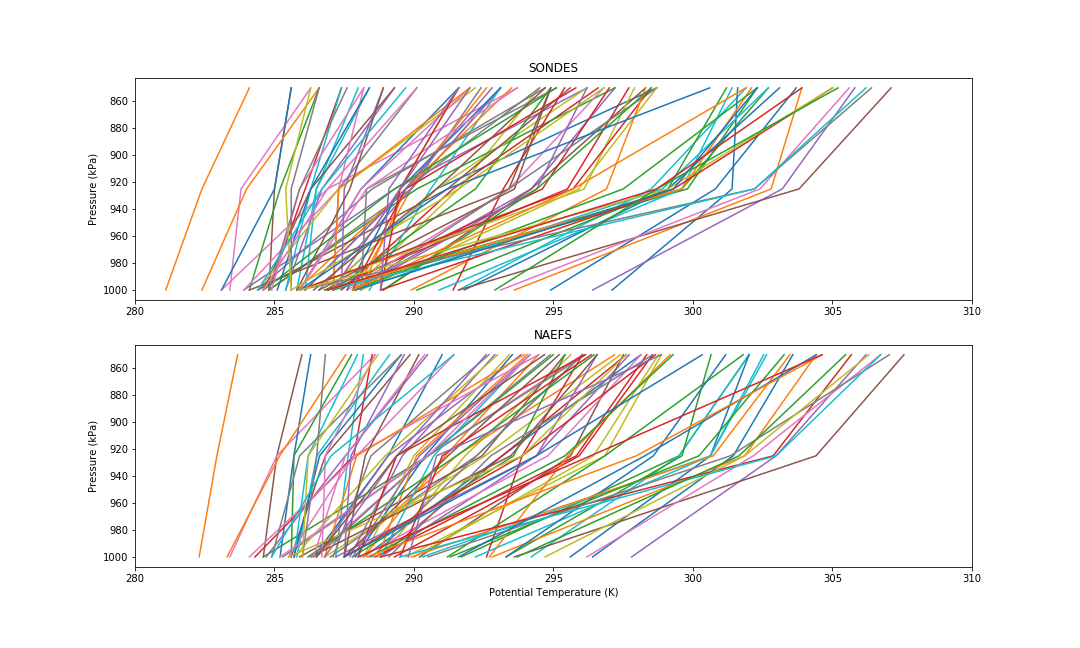
\includegraphics[width=\textwidth]{actual_data_model_v_obs200128.png}
    \caption{Potential temperature at 1000 kPa, 925 kPa and 850 kPa for soundings and NAEFS}
    \label{fig:alldata}
\end{figure}


I use two different data sets for this project: model data and observational data (see Figure ~\ref{fig:alldata}). 
The model data is from the North American Ensemble Forecast System (NAEFS; Government of Canada, 2019; 
archived NAEFS data is available on out team servers). NAEFS is a 42-member ensemble, made up 
of 21 Canadian members and 21 American members. Each group of 21 members comprises one control 
member and 20 perturbed members. The control members are the national weather models for Canada: 
the Global Environmental Multiscale Model (GEM), and for the United States: the Global Forecast 
System Model (GFS). Perturbations in the model are in initial conditions and the physics schemes 
(ECC Canada, 2019). 

For this project I use only one ensemble member: the GFS control member. The model is initialised 
at 00z every day and I use daily forecast runs initialised at this time. The forecasts are 
available for 6-hourly time intervals: 00z, 06z, 12z and 18z. In order to compare model data 
with corresponding observations, I use only the data available at only 00z and 12z. 

The NAEFS models have forecasts for various pressure levels, three of which may able to capture 
the boundary layer, depending on boundary layer height: 1000 kPa, 925 kPa and 850 kPa. Thus, 
these are the levels used in my analysis.


\subsection{Observations}

Observations are from sounding data, available from the University of Wyoming website 
(University of Wyoming, 2019).  Sounding data is generally available at 00z and 12z and 
sometimes for Cape Town it is available at 09z. Soundings record data at many points within 
the PBL. The heights and associated pressure levels at which they are recorded are not 
consistent. In order to compare soundings with model data, I interpolate the soundings 
to the 1000 kPa, 925 kPa and 850 kPa pressure levels. 






\subsection{NAEFS planetary boundary layer scheme}

As discussed earlier, the PBL scheme of any model will determine its ability to forecast 
variables in the boundary layer. What follows will be a brief discussion of the PBL scheme 
used in the Global Forecast System model. 

GFS uses a hybrid Eddy Diffusivity Mass Flux (EDMF) boundary layer parameterization scheme. 
It is hybrid in the sense that different schemes are used under different conditions in 
order to improve forecast accuracy.  This new hybrid scheme was implemented in 2015 in 
order to improve the simulation of PBL growth in the model. The previous scheme that was 
used is an Eddy Diffusivity Counter Gradient (EDCG) scheme, which tended to under estimate 
PBL growth, hence the implementation of the EDMF scheme, which takes into account updraft 
fluxes. However, the EDMF scheme was shown to overestimate mixing in the tropics where the 
PBL is seldom strongly unstable. Thus, the EDCG scheme is still used in these areas as it 
better represents vertical mixing under more stable conditions. The BL scheme is selected 
depending on the stability of the model, making it a hybrid scheme. Stability is determined 
using z/L where L is the Monin-Obukhov stability parameter. The PBL is classified as 
strongly unstable (convective) for z/L $<$ -0.5, and as weakly and moderately unstable 
for 0 $>$ z/L $>$ -0.5, after Sorbjan (1989) (Han et. al., 2016). 


How the two schemes differ:

The two schemes differ in their calculation of the vertical turbulent flux. In the counter 
gradient (CG) scheme the vertical turbulent flux is determined as follows:

EQN 1





\section{Methods}

\section{Results}

\section{Conclusion}

\pagebreak
\section{References}






\end{document}